\documentclass{article}
\usepackage{graphicx} % Required for inserting images
\usepackage{longtable}
\usepackage{amsmath}
\usepackage{subcaption}
\usepackage{url}
\usepackage{hyperref}

\title{Real-Time Visualization of Fluid Simulation \footnote{Inspired by Michel Jean Joseph Donnet's bachelor's degree project \cite{donnetComparaisonEntreMethodes}}}

\author{Michel Jean Joseph Donnet}
\date{December 2025}

\begin{document}

\maketitle

%Headline (General audience)
%Keep it short (ten words or fewer), straightforward, and as free from jargon as you can. For non-specialists, you want to make clear the application/importance of your work, not the specifics (yet!)

\begin{center}
    \textbf{How real-time visualization is a game changer !}
\end{center}

%Summary (General audience)
%This is not an abstract, just a single sentence summing up what you will cover in the article and giving the audience a reason to read on: it should be no longer than 35 words. Try not to repeat the headline in the summary. Please write this section in the third person

\begin{center}
    \textit{The Lattice Boltzmann Method enables real-time visualization of fluid simulations through GPU parallelization thanks to a relevant representation of the fluid
}
\end{center}

%Paragraph 1: The purpose (General audience)
%Give the motivation of your work and its potential applications in a way that the public will be able to understand. 
\paragraph{}{
Water is something that fascinate humans for a long time.
Indeed, Archimedes was already using the properties of fluids for calculations such as the famous legend in which he determined the purity of gold in a crown using the properties of a fluid.
Nowadays, technology has made huge advances, allowing to better understand behavior of fluids thanks to complex simulations.
These simulations are very computationally intensive and require high-end hardware.
However, the development of GPUs (Graphics Processing Unit) and parallel computing on GPUs is making this type of simulation more accessible to a wider audience, particularly in the fields of visual effects, video games, etc.
}

%Paragraph 2: The problem (General technical audience)
%Now give the context of your work for a non-specialist. To what general field or fields (like artificial intelligence or data security) does your work apply, and why is this field important? Describe a goal that researchers in the field have been working towards and problems in achieving this goal (some of which you have solved, or are trying to solve, which you will explain in the rest of the article). Remember to spell out all acronyms the first time you use them, and to explain all jargon terms that aren’t well understood outside your field. 

\paragraph{}{
In general, simulations take place in two stages: computation, then visualization.
Due to the complexity of the calculations, parallelizing fluid simulation is very difficult to achieve, especially on GPUs, which are highly specialized components designed to process large amounts of data in parallel by applying the same calculations to different parts of the data, as is the case in image and video processing, for example. %which have a specific structure that only accepts certain types of tasks but offer high computing power. %which are highly specialized components designed to process large amounts of data in parallel by applying the same calculations to different parts of the data, as is the case in image and video processing, for example.
That's why most methods perform parallelization on CPUs (central processing units) rather than GPUs due to the complexity of exploiting parallelization on GPUs.
}

%Paragraph 3: The set up (General technical audience)
%From the issues you described in the first paragraph, now pick out the ones that concern your work. How have people tried to solve this/these in the past? Why have these solutions fallen short? What is (briefly) your new solution?

\paragraph{}{
%Some approaches to perform both visualization and computation by exploiting parallelization on GPUs to save computation time, such as the method based on NVIDIA's GVDB Voxel technology \cite{Wu:2018:gvdb_flip}, which uses the specific architecture of NVIDIA GPUs to perform computation and visualization in parallel.
Some approaches that enable both visualization and computation by exploiting parallelization on GPUs have already been implemented, such as the method based on NVIDIA's GVDB Voxel technology \cite{wuFastFluidSimulations2018}, which uses the specific architecture of NVIDIA GPUs to perform computation and visualization in parallel.
Other methods, designed more for visual results than for simulation realism, have been developed, particularly in game engines such as Fluid Flux for Unreal Engine \cite{FluidFluxDocumentation}.
The proposed method will attempt to address the challenges posed by GPU parallelization and fluid simulation in a novel way, using fluid modeling that facilitates GPU usage.
} 

%Paragraph 4: Your approach (Audience in your discipline)
%Having mentioned your approach in the last paragraph, you should now explain the basic concepts behind it and how it works. Here you can be a little more technical, but if you use words that can’t be looked up in a basic scientific dictionary, add some explanation. 

\paragraph{}{
The new method developed and implemented by Dr. Moritz Lehmann \cite{lehmannHighPerformanceFree2021a}, called the lattice Boltzmann method (LBM), is not based on the famous Navier-Stokes equations, which represent the flow of a viscous fluid.
Indeed, these equations are very complex and have no known mathematical solution to date: the Navier-Stokes equations are among the \textit{Millennium Prize Problems} for which a reward of one million dollars is offered to anyone who can solve them.
The approach used is derived from the \textit{Lattice Gaz Automata} method developed in 1973 by J. Hardy, Y. Pomeau, and O. Pazzis \cite{Hardy1973TimeEO}, which uses Boltzmann equations instead of Navier-Stokes equations.
In contrast to the Navier-Stokes equations, which describe the behavior of fluids at a macroscopic level, Boltzmann's equations use a microscopic representation of the fluid in the form of a set of populations of particles that interact with each other as shown on figure \ref{fig:lattice}.
}

\begin{figure}[ht]
    \centering
    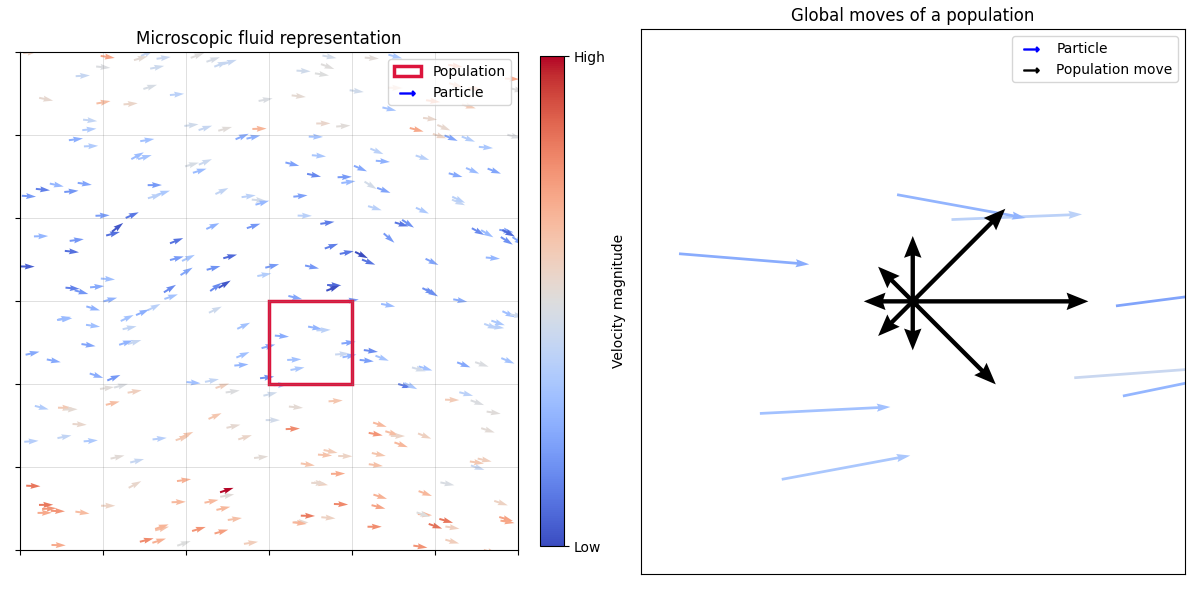
\includegraphics[width=0.7\textwidth]{img/graph.png}
    \caption{Lattice vectors used in the simulation}
    \label{fig:lattice}
\end{figure}


%Paragraphs 5-7: What you’ve done (Audience in your discipline for paragraph 5, moving to a specialist audience for 6 and 7)
%This is the most straightforward section of the article, and the one that is least likely to be a problem. Go through what you’ve done, what your results were, and what your results mean. Just start off on the less technical side so that those that aren’t right in your field can grasp the basics what you’re trying to do: even if they don’t understand the full details as you progress

\paragraph{}{
As in Boltzmann's equations, the LBM method defines a distribution function $f(\xi, \mathbf{x}, t)$ \footnote{Note that in the literature, since we are working with discrete $\xi_i$ due to the population decomposition, $f(\xi_i, \mathbf{x}, t)$ can also be written as $f_i(\mathbf{x}, t)$.} that describes the number of particles at position $\mathbf{x}$ at time $t$ moving in direction $\xi$ at velocity $\lVert \xi \rVert_{2}$ \footnote{All variables descriptions can be found in Table \ref{tbl-var-clean} in Appendix}.
The main difference here is that the LBM method works with particle populations instead of considering each particle separately, which is computationally intensive.
The distribution function $f$ is normalized such that integration over velocity and position gives the mass of the population, as shown in equation (\ref{eq:mass}), to ensure that the Euler's principle of conservation of mass is respected.
Indeed, when the velocity and position of each particle are neglected, only the mass of the population remains.
\begin{equation}
    \label{eq:mass}
    \int d^3 \xi \int d^3 \mathbf{x} f(\xi, \mathbf{x}, t) = M(t)
\end{equation}

Calculating the moments of the distribution function $f$ enables the characteristics of the fluid to be extracted, such as the particle density $\rho$ for moment 0 or the momentum $\rho u$ for moment 1.
The function $f$ evolves over time as described in equation (\ref{eq:evolution}), in accordance with Newton's second law.
\begin{equation}
\label{eq:evolution}
\begin{aligned}
\frac{df(\xi, \mathbf{x}, t)}{dt}
&= \left(\frac{dt}{dt} \cdot \frac{\partial}{\partial t} + \frac{d\mathbf{x}}{dt}\cdot \frac{\partial}{\partial \mathbf{x}} + \frac{d\xi}{dt} \cdot \frac{\partial}{\partial \xi}\right) f(\xi, \mathbf{x}, t) \\
&= \left(\frac{\partial}{\partial t} + \xi \cdot \frac{\partial}{\partial \mathbf{x}} + \frac{F}{\rho} \cdot \frac{\partial}{\partial \xi}\right) f(\xi, \mathbf{x}, t) \\
&= \frac{\partial}{\partial t}f + \xi \cdot \nabla_{\mathbf{x}} f + \frac{F}{\rho} \cdot \nabla_{\xi}f \\
\end{aligned}
\end{equation}
The collision operator $\Omega$ can then be defined as the relaxation of the function $f$ towards the equilibrium function $f^{eq}$ (defined in equation (\ref{eq:equilibrum})) thanks to the work of Bhatnagar, Gross, and Krook\cite{Bhatnagar}, with $\tau$ being the relaxation time as indicated in equation (\ref{eq:relaxation}).
\begin{equation}
\label{eq:relaxation}
\Omega (f) =- \frac{1}{\tau} (f - f^{eq})
\end{equation}
\begin{equation}
\label{eq:equilibrum}
f^{eq} (\xi, \mathbf{x}, t) = \rho \left(\frac{1}{2\pi RT}\right)^{3/2} e^{-\frac{|\xi|^2}{2RT}}
\end{equation}

\begin{figure}[ht!]
    \centering
    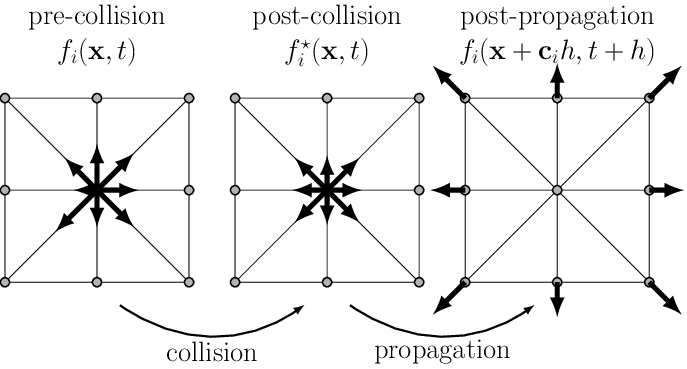
\includegraphics[width=0.7\textwidth]{img/algo.png}
    \caption{Taken from work of Schiller, Ulf and Krüger, Timm and Henrich, and Oliver \cite{algo}}
    \label{fig:propagation}
\end{figure}

As shown in Figure \ref{fig:propagation}, the algorithm operates in two main steps: collision calculation, followed by propagation of the result to neighboring particle populations.
In this way, interactions are local and can be exploited for GPU parallelization.
The implementation, benchmarks, documentation, and examples are available on ProjectPhysX/FluidX3D on GitHub \cite{Lehmann_FluidX3D_2022}.
GPU parallelization is effective and enables realistic real-time rendering of fluid simulations, as shown in Figure \ref{fig:ex1}.
For more complex cases, the simulation can be run on multiple GPUs from different manufacturers, as shown in Figure \ref{fig:ex2}.
However, real-time visualization is not possible and the simulation must be saved.
}

\begin{figure}[h!]
    \centering
    \begin{subfigure}[b]{0.45\textwidth}
        \centering
        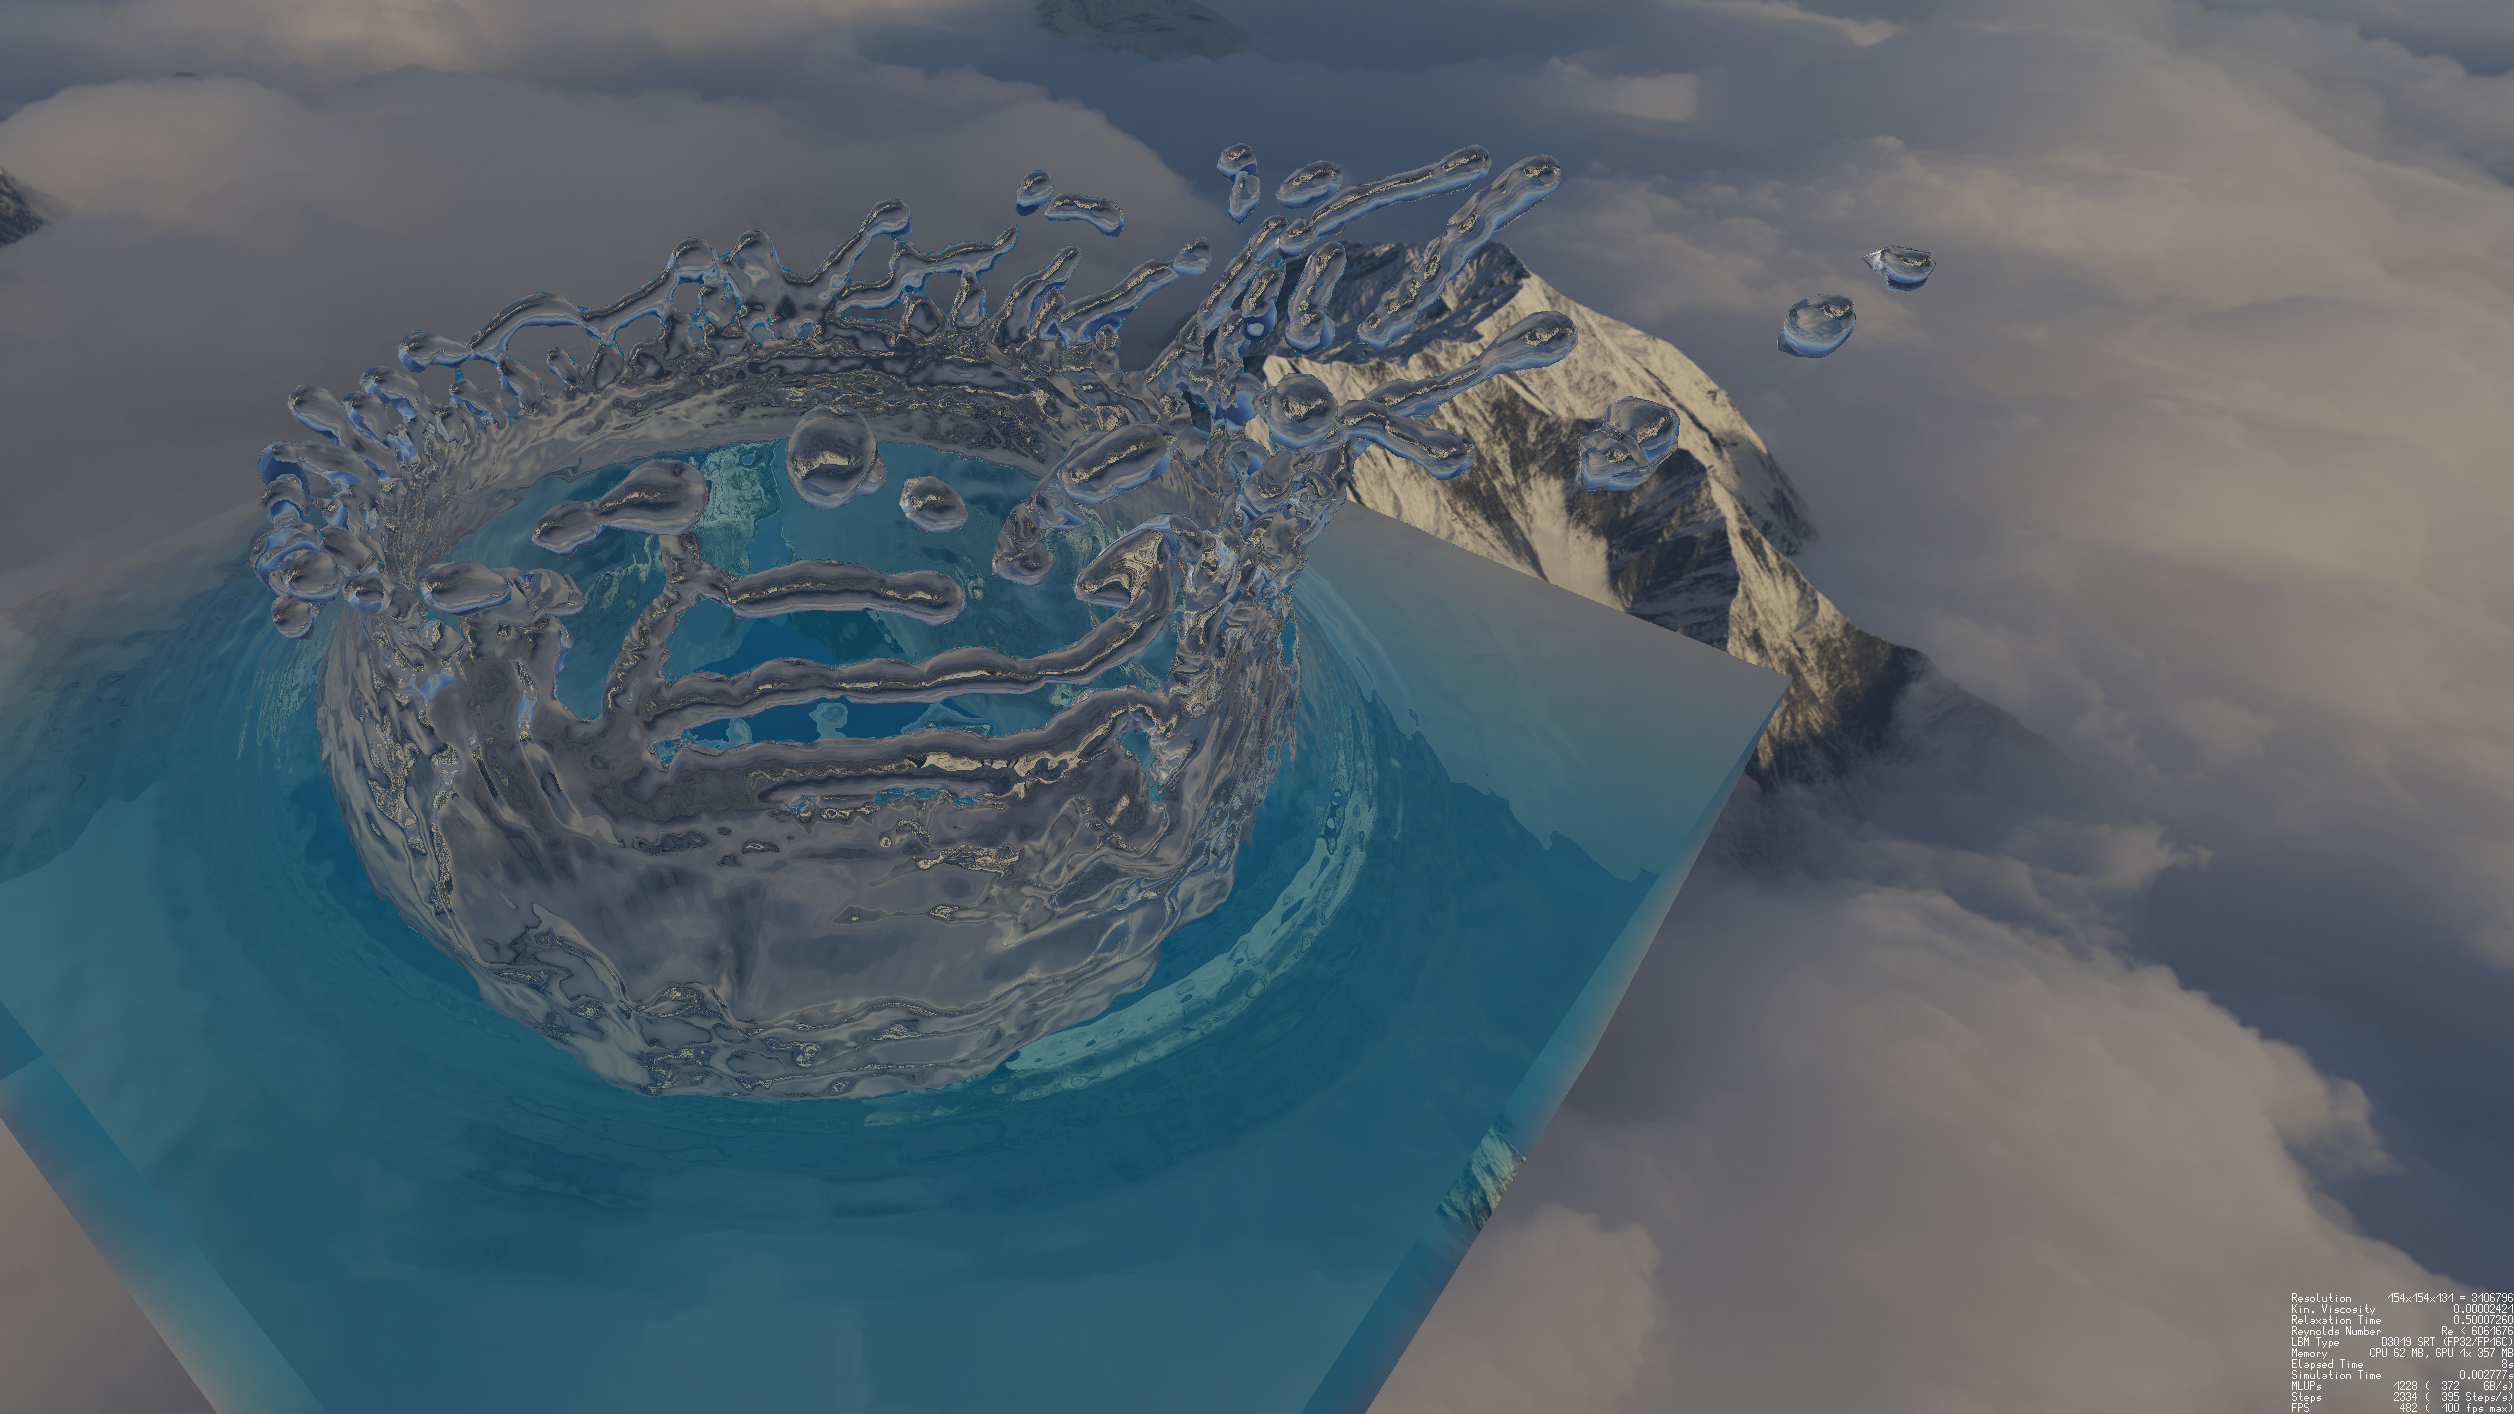
\includegraphics[width=\textwidth]{img/example.png}
        \caption{Real-time visualization with a resolution grid of 3 million cells}
        \label{fig:ex1}
    \end{subfigure}
    \hfill
    \begin{subfigure}[b]{0.45\textwidth}
        \centering
        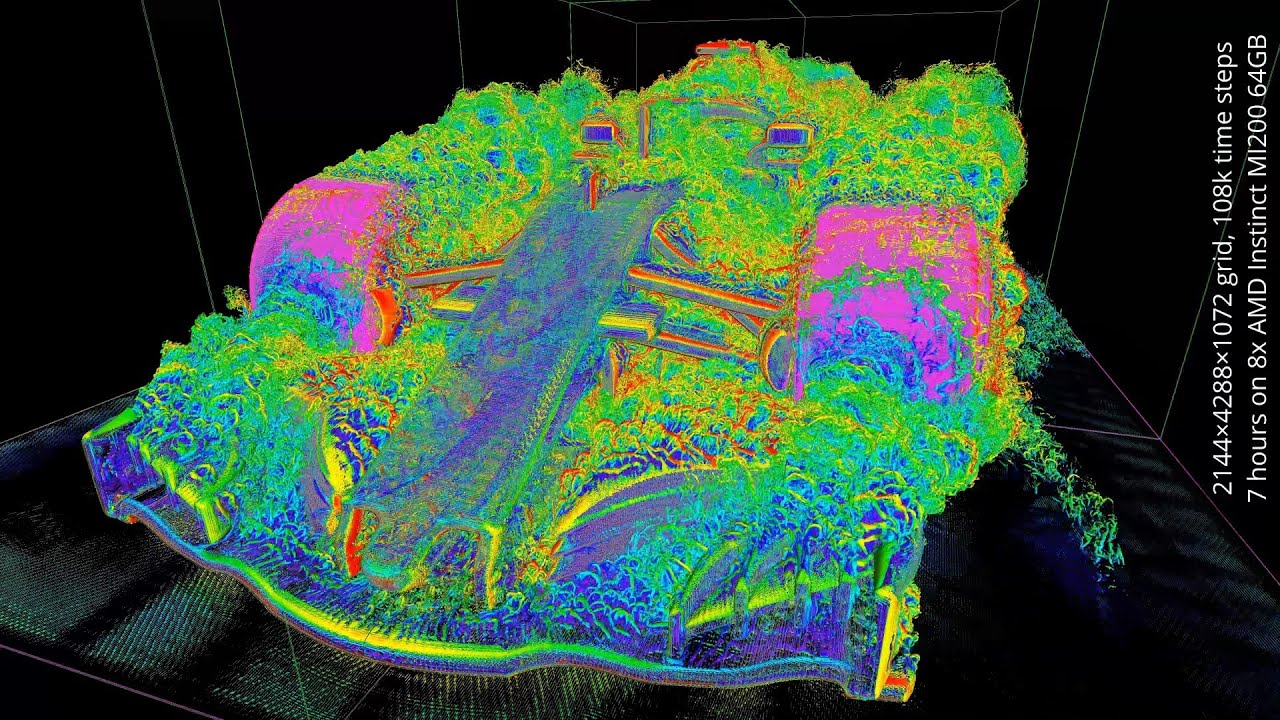
\includegraphics[width=\textwidth]{img/backing_example_2.jpg}
        \caption{Fluid simulation with a resolution of 1 billion cells}
        \label{fig:ex2}
    \end{subfigure}
    \caption{Results of Lattice Boltzmann Method}
    \label{fig:both_images}
\end{figure}




%Paragraph 8: Conclusion/further work (General technical audience)
%Go back and remind us of the application, the problem with it (without restating from scratch), and explain how the work you’ve just described has moved things on. Then tell us how you think you can make even further progress.

\paragraph{}{
In conclusion, by approaching fluid simulation from a different angle, the Lattice Boltzmann Method allows for extensive parallelization of fluid simulation across multiple GPUs, with the possibility of real-time visualization when running on a single GPU.
A next step could be to enable real-time simulation rendering on multiple GPUs, or to use a sparse volumetric representation of the data on the GPU to enable simulation with an adaptive domain and increase simulation efficiency by using less data on the GPU, or to implement the Lattice Boltzmann method in 3D software such as Blender. \footnote{English correction performed by DeepL}
}

\section*{Appendix}

\begin{table}[h]
\centering
\caption{Variables appearing in the governing equations}
\label{tbl-var-clean}
\begin{longtable}{|c|c|c|}
\hline
\textbf{Variable} & \textbf{Description} & \textbf{Unit} \\
\hline
\hline
$t$ & Time & $s$ \\
$\mathbf{x}$ & Particle position & $m$ \\
$\xi$ & Particle velocity. Can be defined as $\xi = \frac{d\mathbf{x}}{dt}$ & $m \cdot s^{-1}$ \\
$f$ & Particle distribution function & $m^{-3} \cdot s^{3}$ \\
$f^{eq}$ & Equilibrium distribution function & $m^{-3} \cdot s^{3}$ \\
$\rho$ & Fluid density & $kg \cdot m^{-3}$ \\
$F$ & External force & $N$ \\
$\tau$ & Relaxation time & $s$ \\
$R$ & Specific gas constant & $J \cdot kg^{-1} \cdot K^{-1}$ \\
$T$ & Temperature & $K$ \\
$M(t)$ & Total mass of the system & $kg$ \\
\hline
\end{longtable}
\end{table}




\pagebreak

\bibliographystyle{plainurl}
\bibliography{main-bib}

\end{document}
